\section{Result And Discussion}

\begin{table}[]
	\caption{Target type detection performance.}
	\scalebox{0.7}{
		\begin{tabular}{c|c|c|c}\label{results}
			
			Feature Group                               & Retrieval model                & NDCG@1   & NDCG@5   \\ \hline
			Entity Centric                              & \multirow{2}{*}{Probabilistic} & 0.1490   & 0.3223   \\ 
			Type Centric                                &                                & 0.2341   & 0.3780   \\ \hline
			Entity Centric                              & \multirow{2}{*}{FeedForward}  & 0.1886*  & 0.3289   \\ 
			Type Centric                                &                                & 0.2786*  & 0.4011*  \\ \hline
			Entity Centric                              & \multirow{2}{*}{CNN}      & 0.3341** & 0.4586** \\ 
			Type Centric                                &                                & 0.4034** & 0.5287** \\ \hline
			Entity + Type                               & CNN                       & 0.4575   & 0.5994   \\ \hline
			Entity + Type + Knowledge Base + Type Label & LTR                            & 0.4842   & 0.6355   \\ \hline
		\end{tabular}
	}
\end{table}

\begin{figure*}
	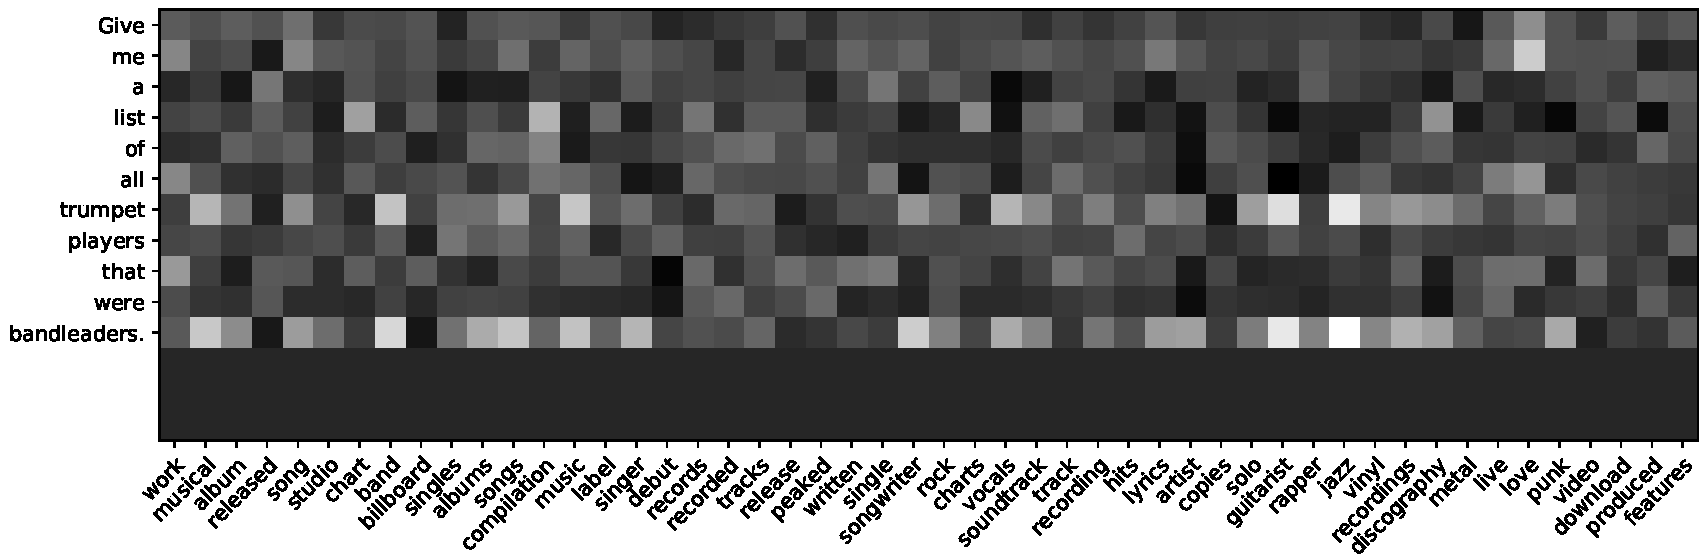
\includegraphics[width=\textwidth]{leaders_in_cropped.pdf} \caption{input of type centric CNN model}\label{conv1Input}
	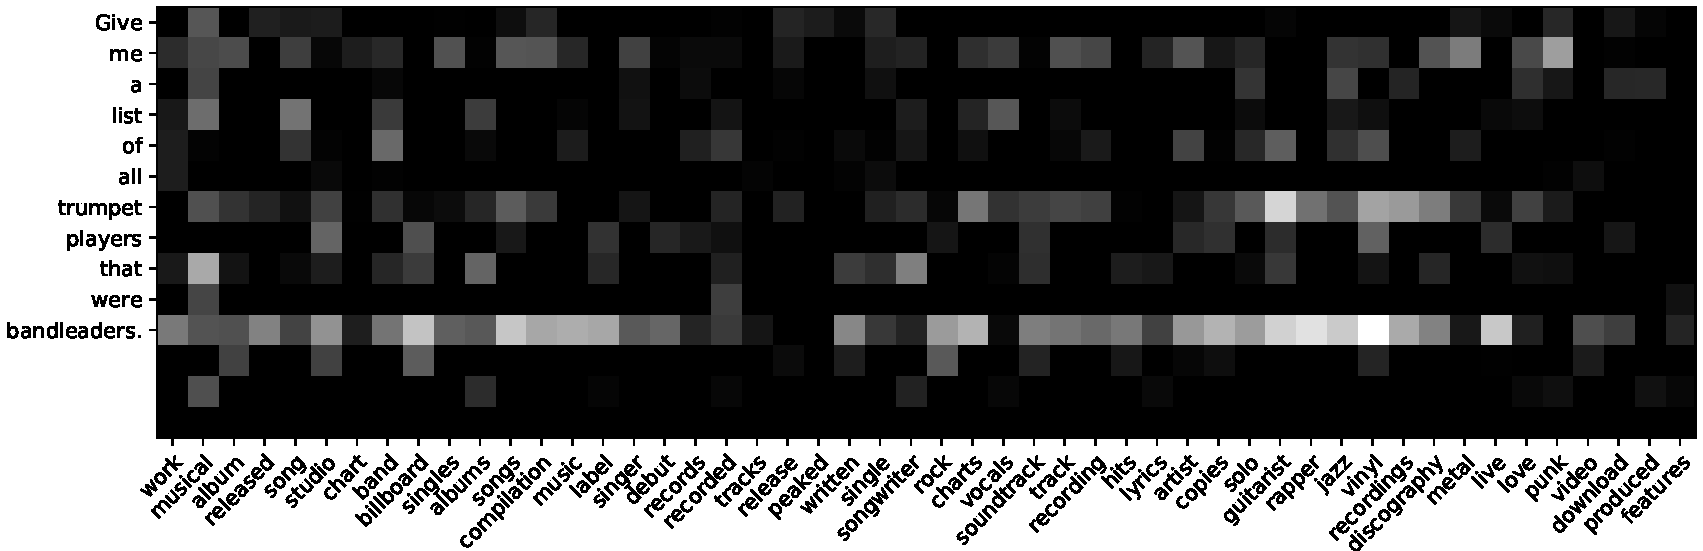
\includegraphics[width=\textwidth]{leaders_conv1_cropped.pdf}
	\caption{output of type centric CNN model after conv1 layer}\label{conv1Output}

\end{figure*}



Table \ref{results} presents the evaluation results. We find that the feedforward network significantly (except Entity Centric for NDCG@5 measure) outperforms the probabilistic model both in the entity and type centric approaches. significant improvement is measured with $p$<0.05 using two-tailed pair-test. In addition, the CNN architecture improves the feedforward network significantly by a large margin both in entity centric and type centric approaches. Another interesting observation here is that the hybrid model (i.e entity + type centric) can improve the NDCG@1 and NDCG@5 significantly.

The interesting observation here is that the NDCG@1 of CNN model (in hybrid setting) is not worse than the LTR model significantly. In other words, although, the LTR model utilizes several hand-crafted features, it can not outperform the CNN proposed model.

In order to better analyze the behavior of CNN network, we visualized the input of $I_{TC}$ and the output of first convolution layer for the query \textit{"Give me a list of all trumpet players that were bandleaders."} and type \textit{"MusicalArtist"} in fig.\ref{conv1Input} and fig.\ref{conv1Output} respectively. As indicated in these figures the horizontal axis indicates top-50 words representing \textit{MusicalArtist} type sorted by tf.idf from left to right. in this figure, lighter entries indicate the larger value of similarity between a query term and the corresponding representing term. By comparing the output and output matrices, we find that the CNN model is able to remove noises i.e non-relevant terms to that specific type. for example the weights associated with query terms "\textit{give}" and "\textit{me}" are reduced significantly. According to this observation, CNN network outperforms the FF because it can extract local features (by local we means the feature associated with the context of query) while the FF network only uses the word2vec embedding of each word and that not consider it's context in the query. our proposed model is an economic model because we don't use any complicated features, but it can capture the relationship between the query and it's target type effectively.     





\begin{figure}
    \scalebox{.45}{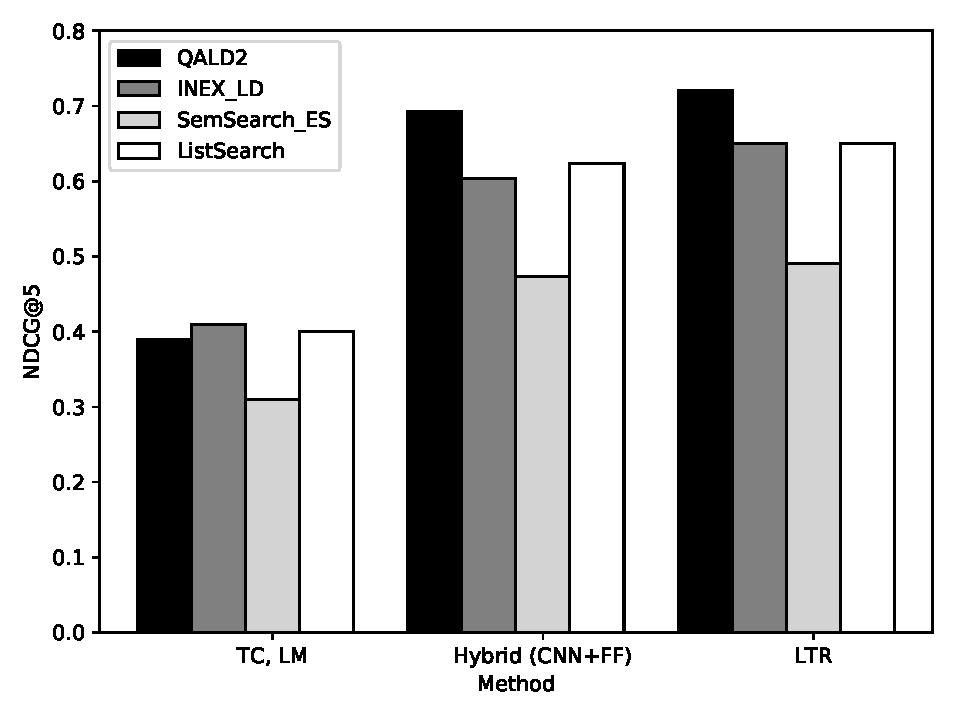
\includegraphics[]{categorize_analyze.pdf}}
	
	\caption{Performance across queries based on query categories}

\end{figure}

\subsection{Conclusion}
Target type identification is an important problem in entity retrieval, it can enhance the performance of entity retrieval for entity-bearing queries. In this paper we propose a convolutional neural network architecture to capture local features of entity bearing queries. Our experiments indicate that the proposed architecture outperform simple feedforward network as well as probabilistic (TC, EC) models. Our architecture considers the order of query terms as well as the order of top-k terms representing entities and types. several layers of CNN extract important features to solve this problem. Our interesting observation is that LTR model with a rich set of hand-crafted features can only slightly perform better than the CNN.

